\documentclass[12pt]{article}

%% EXCLUSIVE PACKAGES
\usepackage[utf8]{inputenc}
\usepackage[affil-it]{authblk}
\usepackage[dvipsnames]{xcolor}

\usepackage{epigraph}
\setlength\epigraphwidth{.8\textwidth}
\setlength\epigraphrule{0pt}

\usepackage{array}

\usepackage{biblatex}
\addbibresource{biblio.bib}


\usepackage{TheoStyle}

\title{\textbf{Patterns Analysis in Coupled Parabolic-ODE Systems}}
\author{Théo ANDRÉ}
\affil{Turing Center For Living Systems \& Aix-Marseille Université}

\date{January 2023 - July 2023}

\color{lightgray}
\pagecolor{black}

% EXCLUSIVE DEFS
\def\uu{\bm{u}}
\def\vv{\bm{v}}
\def\ww{\bm{w}}

\begin{document}

% LE TITRE
\maketitle


% ABSTRACT
\begin{abstract}
    This thesis builds upon previous work pioneered by Anna Marciniak-Czochra in using coupled reaction-diffusion equations to ODE to model pattern formation in Hydra, a freshwater polyp known for its regenerative abilities. Previous studies have shown that such models can successfully capture the emergence of spatial patterns of gene expression during regeneration, and have identified key signaling molecules such as Wnt and Notch as playing a critical role in this process. However, these models have largely ignored the physical properties of the tissues in which regeneration occurs. In this thesis, we come back to the model presented in \cite{AnnaThesis} that integrates coupled reaction-diffusion to ODE models and see if we can reduce the amount of parameters, exhibit hysteresis and investigate the phenomenon of Turing Patterns / Far-From-Equilibrium patterns. Ultimately, this thesis aims to provide classical results on the topic and use these notions to further extend the analysis of the model.
\end{abstract}

\vspace{30pt}

\begin{remark}[Color code for Editing] Each color has a meaning: 
	\bigskip
	
	\com{Pink text:} A remark / Comment: \texttt{\textbackslash com\{ ...\}}
	\bigskip
	
	\incl{Green text: } Potential text to include but has the wrong formulation: \texttt{\textbackslash incl\{ ...\}}
	\bigskip
	
	\bref{Blue text:} A reference that is missing and has to be included in the bibliography : \texttt{\textbackslash bref\{ ...\}}
\end{remark}

\newpage

% LA TABLE DES MATIÈRES
\tableofcontents
\bigskip\bigskip

\url{https://www.youtube.com/watch?v=6rr5oLEjMmY} : How to collect polyps and medusae

\url{https://youtu.be/hmkeZ7_6owI} : Hydra morphogenesis symposium



\newpage


% QUOTE

		\epigraph{``In the 300 years since Newton, mankind has come to realize that the laws of physics are always expressed in the language of differential equations''}{--- \textit{Steven Strogatz}}


% DOCUMENT

\section{Notations}

In the entirety of the thesis, we use the following naming conventions

\begin{itemize}
    \item $u$: the amount of free receptors
    \item $v$: the amount of ligands
    \item $w$: the amount of enzymes
    \item $X = (u, v, w) \in \R^3$: the information vector of each quantity in the system
    \item $\Delta$: The Neumann Laplace operator defined by $\Delta f = \sum_{j = 1}^n \frac{\del^2 f}{\del x_j^2}$ with domain $$\euD(\Delta) = \lc f \in \bigcap_{p\ge 1} W_{loc}^{2, p}(\Omega) : f, \Delta f \in \mathcal{C}(\Omega) \text{ and } \frac{\del f}{\del \nu} = 0 \text{ on } \del\Omega \rc$$
    \com{this notation is the one from \cite{Cygan2022}, maybe it is too sophisticaed for this thesis}
\end{itemize}
% TALK ABOUT HYDRA AND HOW THE ORGANISMS CAN REGENERATE PARTS OF ITS BODY.

\section{Hydra Morphogenesis and regenerative properties}

\subsection{Anatomy of a Hydra}

Hydras are fascinating organisms. Despite their rather small size (roughly 5mm of length in average), they are capable of extraordinary regenerative properties that allows them to fully reconstruct their body out of a very small portion of tissue (see figure \ref{hydraregen}).
\begin{figure}
\label{hydraregen}
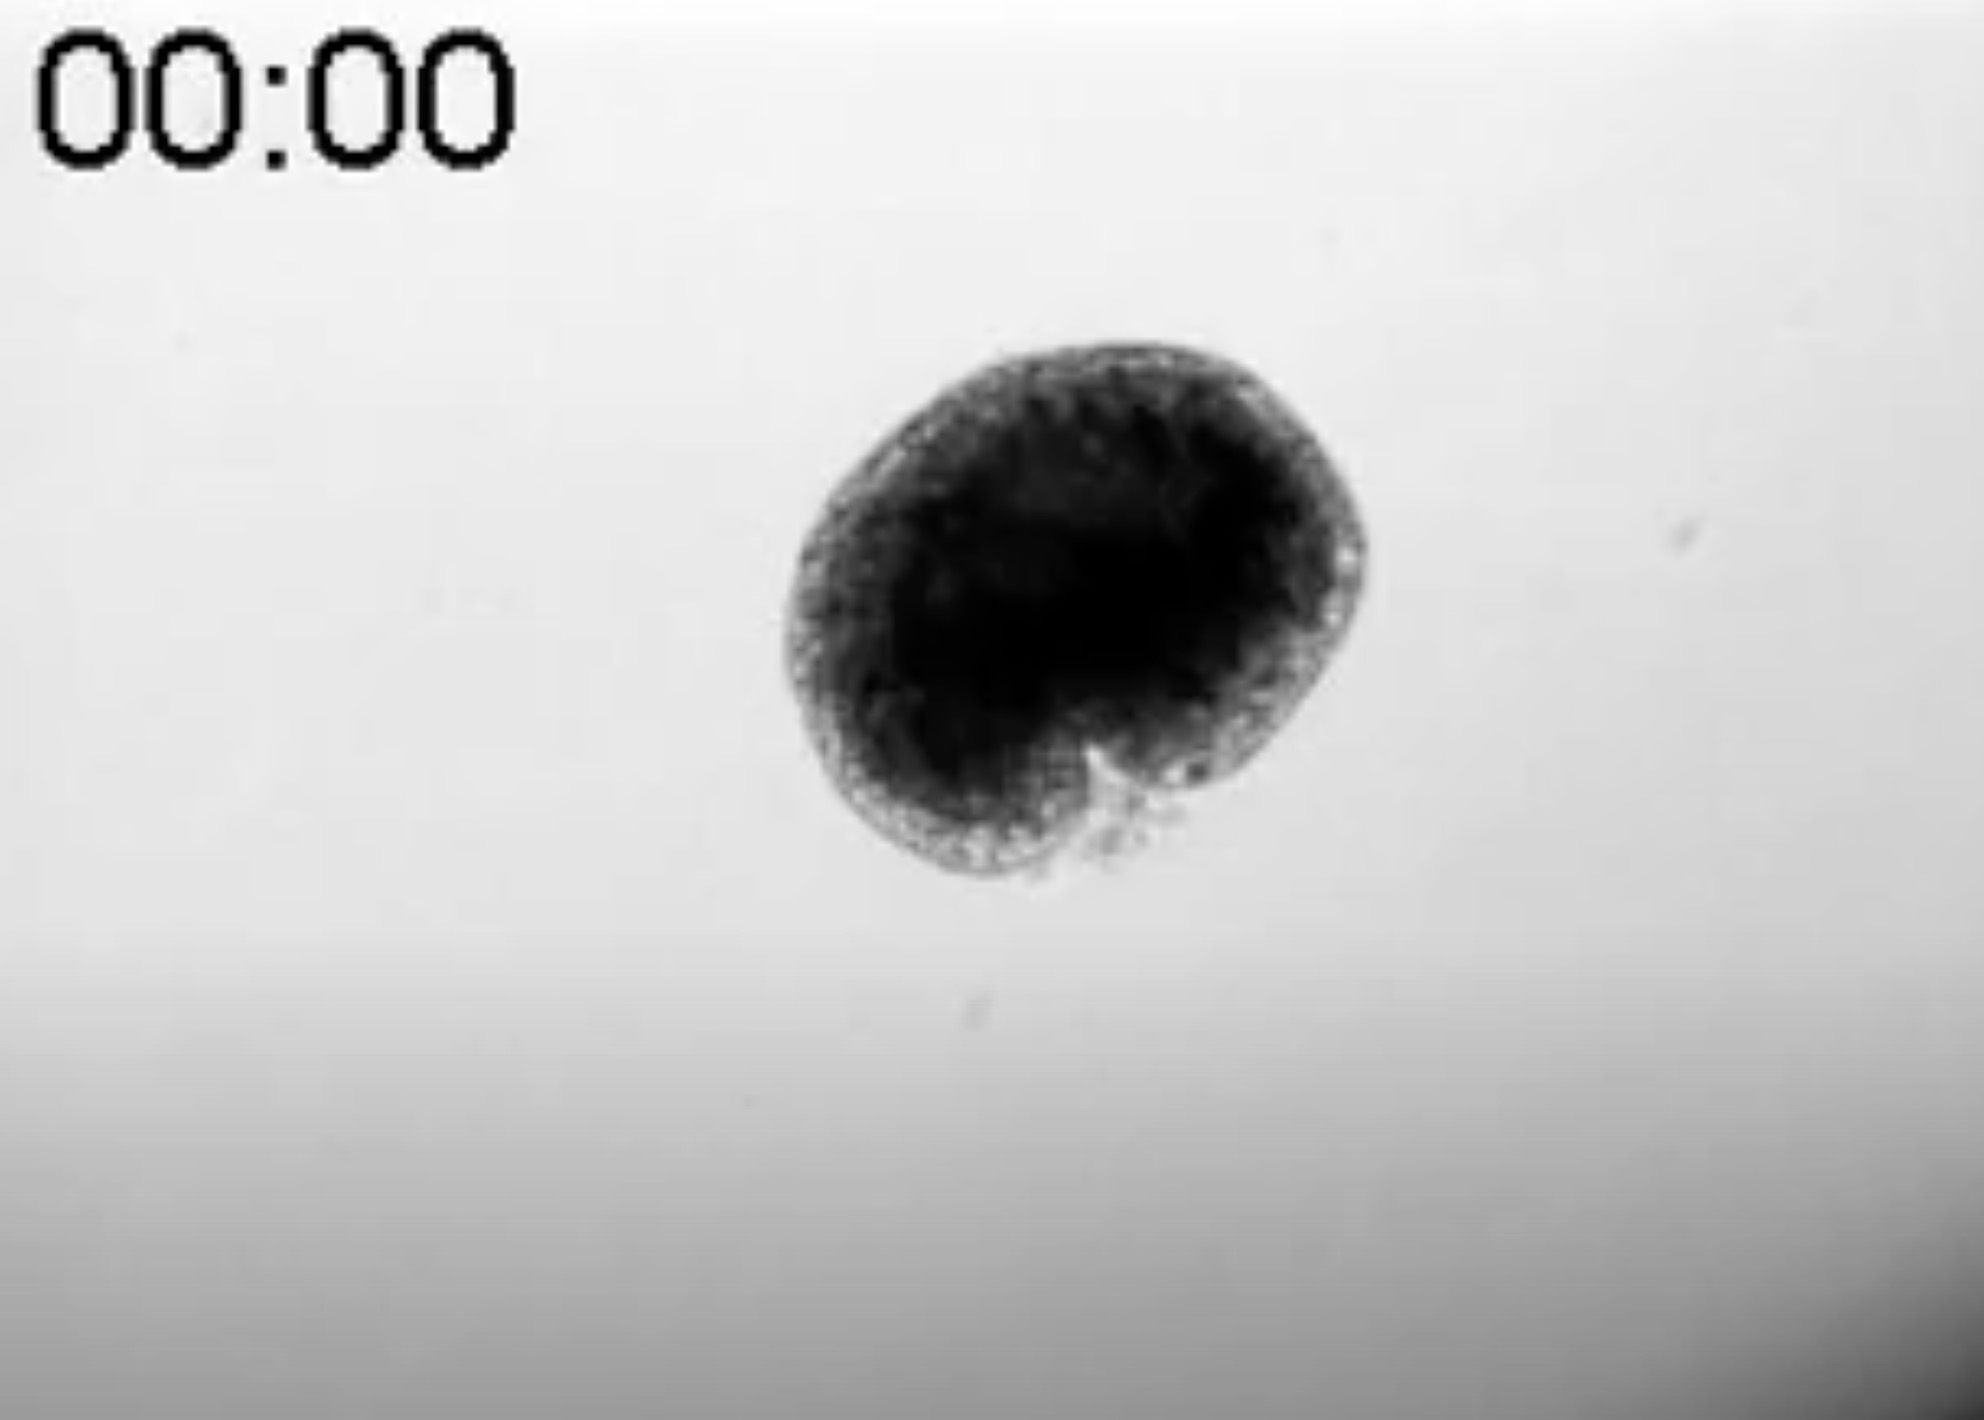
\includegraphics[width=0.19\textwidth]{figures/hydra_growth1}
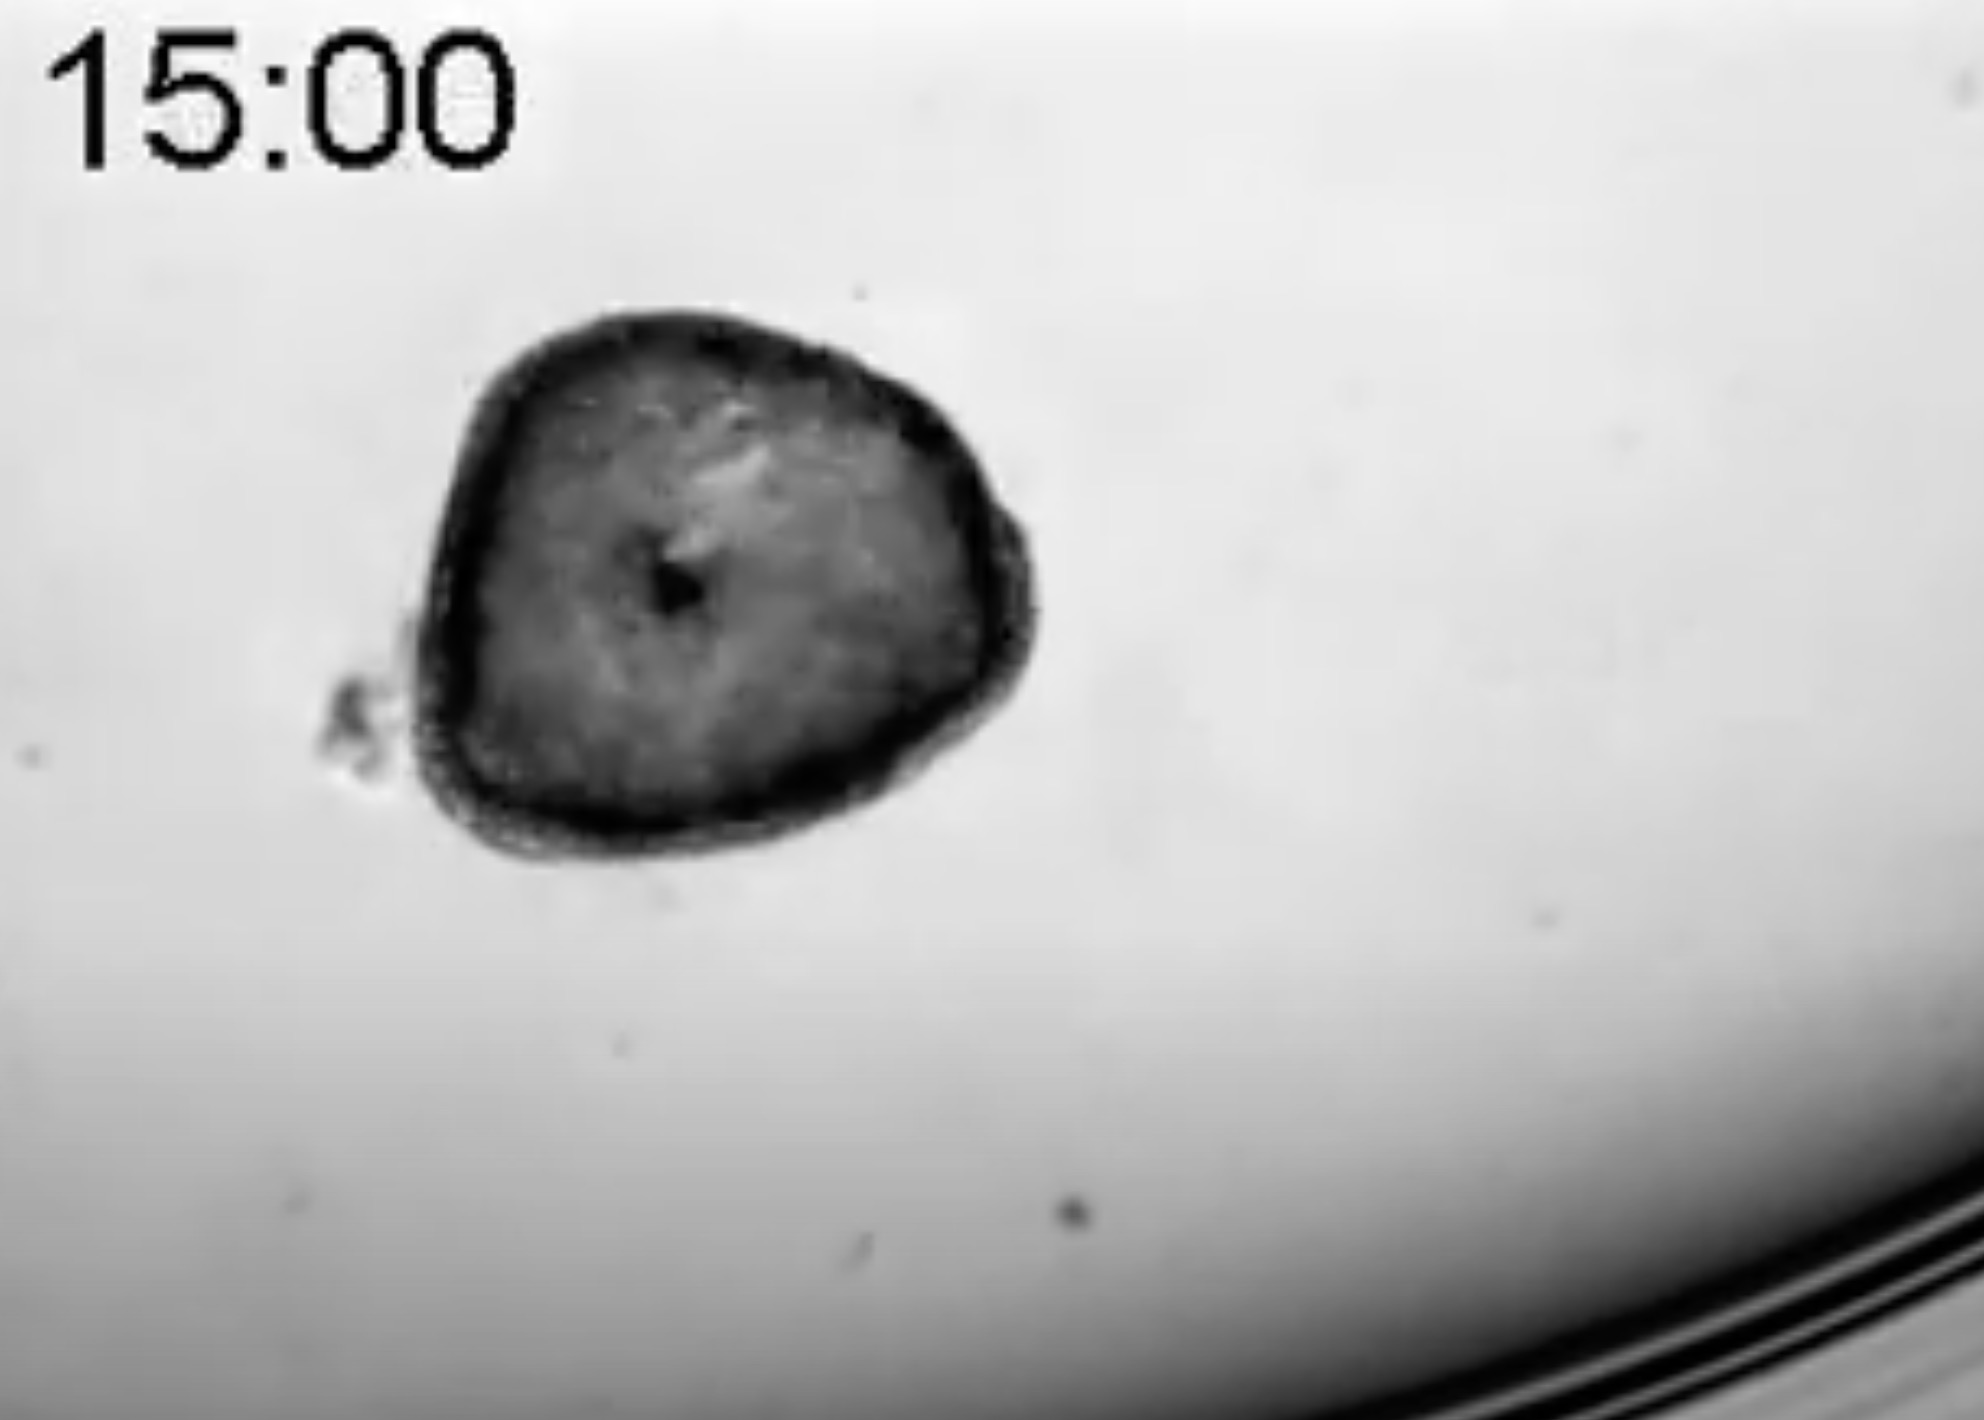
\includegraphics[width=0.19\textwidth]{figures/hydra_growth2}
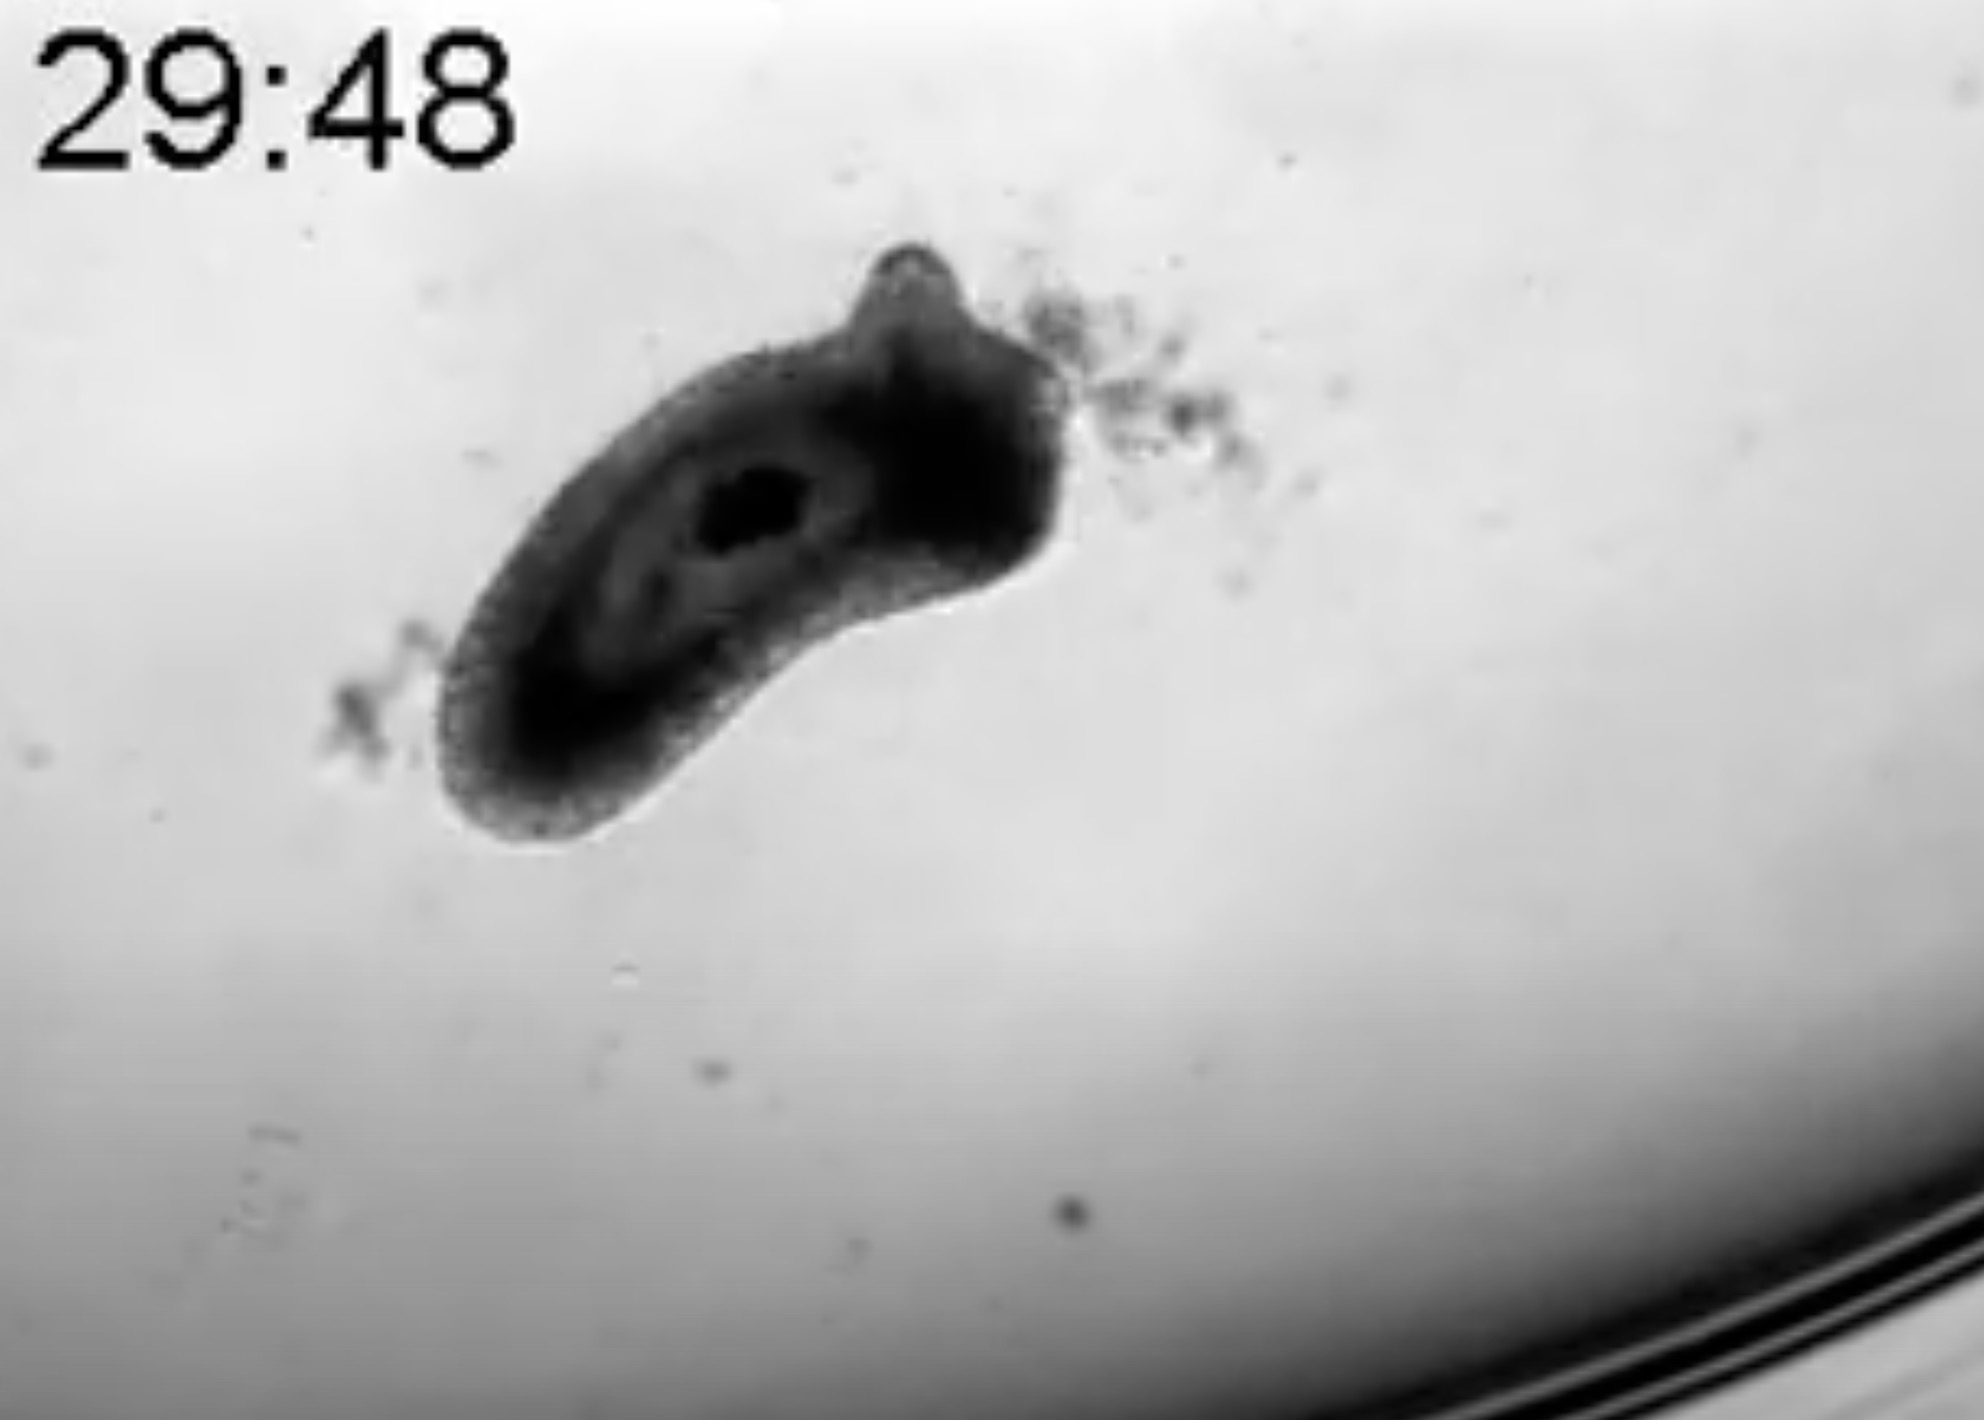
\includegraphics[width=0.19\textwidth]{figures/hydra_growth3}	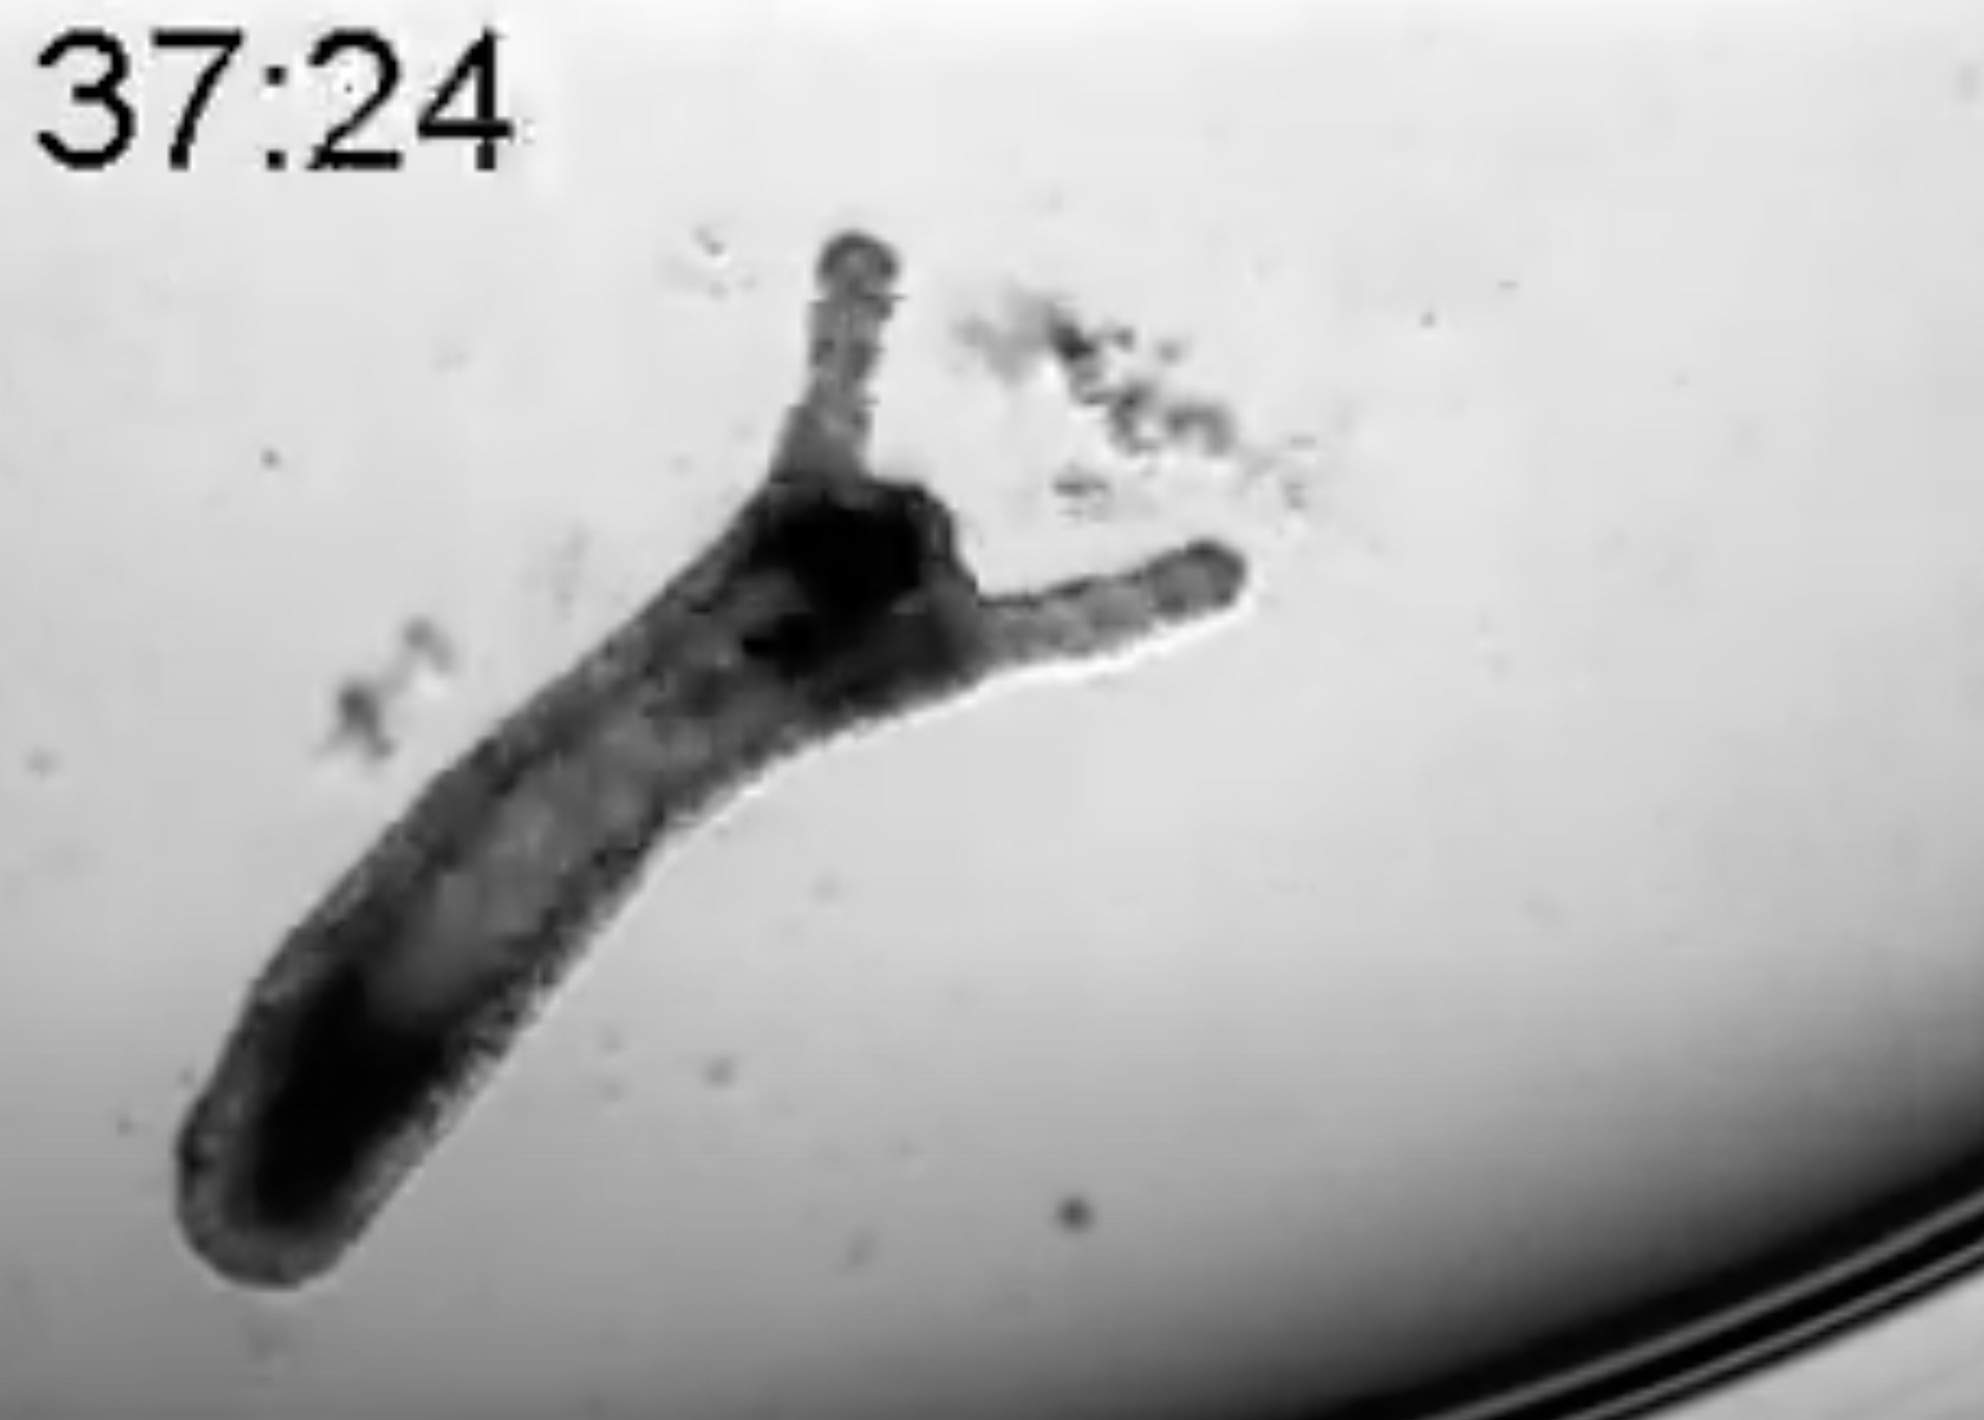
\includegraphics[width=0.19\textwidth]{figures/hydra_growth4}
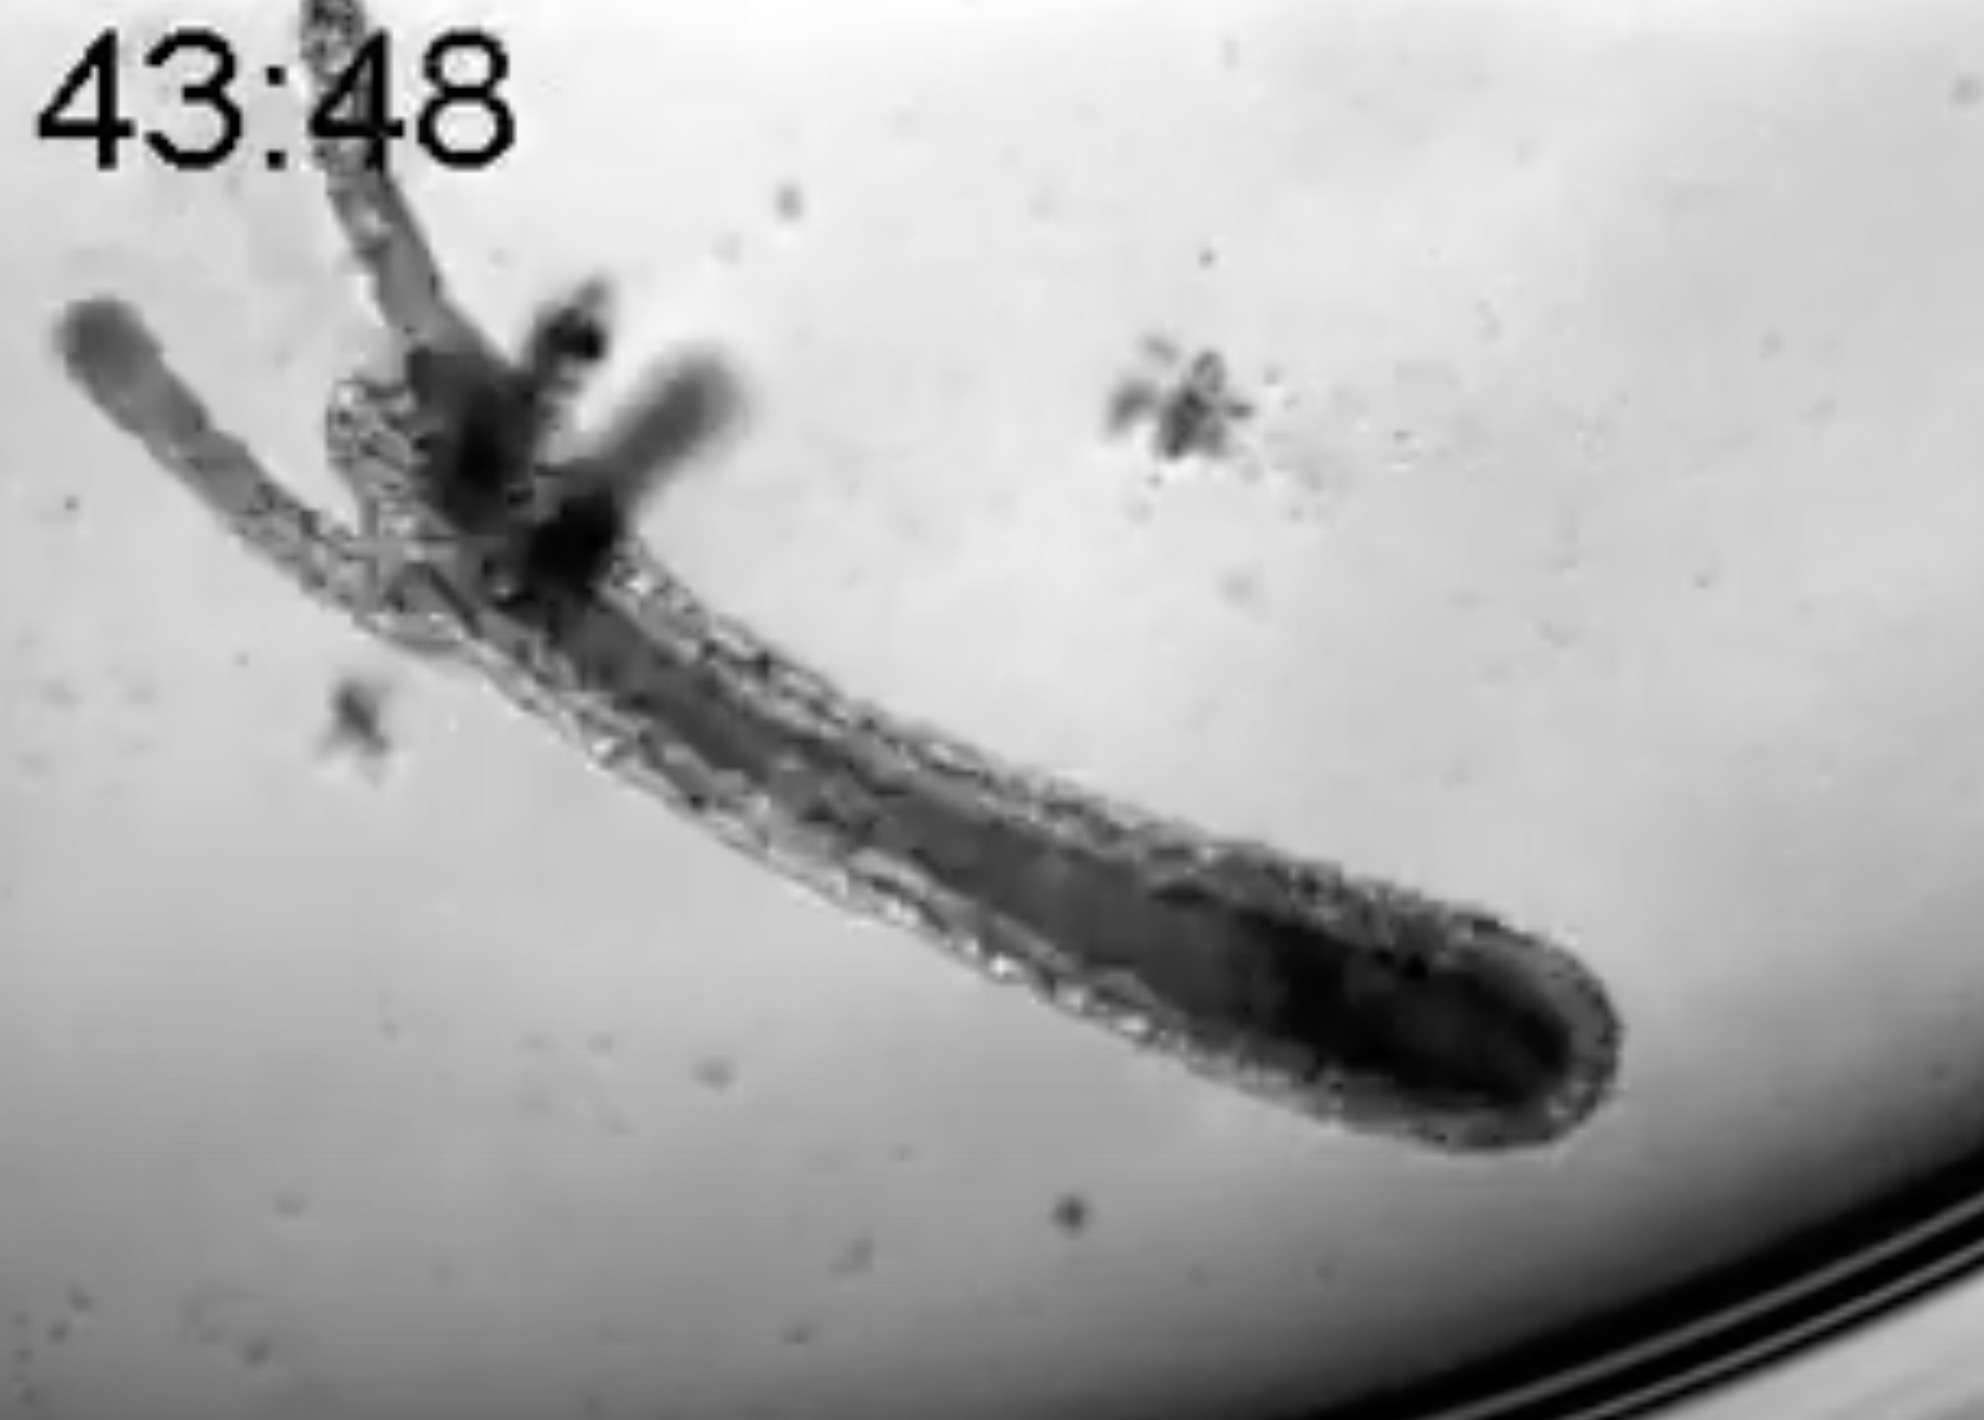
\includegraphics[width=0.19\textwidth]{figures/hydra_growth5}
\caption{Sequence of pictures taken under a traditional microscope. It shows how a Hydra is capable of regenerating its entire body from a small extracted sample of tissue coming from the body column (tissue diameter about 100 $\mu$m) of another Hydra. The timestamp on each picture is formatted as "hours:minutes", meaning the entire regeneration process takes place within the span of two days only.}
\end{figure}

Their body is composed of essentially three regions: the head, body column and foot. Spatially speaking, the small cnidarian is symmetrically organized around the oral-aboral axis giving it its hollow, tubular shape. Taking a step closer on each parts, one can notice that the head is composed of two sub-regions, one being a set of tentacles while the other one is called hypostome and acts as a mouth (it is also the only orifice in the whole organism). The foot, on the other hand is composed of a basal disc that allows hydras to stick to leaves and rocks - among others - underwater. Lastly, the body column is a long hollow tube made of cells undergoing constant mitosis through the life of the polyp. This ensures a constant cellular turnover of the derm (+ add why is it good). 

\subsection{Hydra reproduction and selection}

The way Hydras reproduce is very beneficial to the scientific community since they are able to reproduce either sexually or asexually (with the second one being the most common way of reproduction). The main difference between these two methods is that asexual reproduction preserves the totality of information in one individual, letting one the ability to "keep" a specific Hydra with nice genetic information for further reproduction. It is possible to repeatedly multiply a specific organism through asexual reproduction yielding   

\subsection{The importance of Wnt signaling}

\section{Emergence of Patterns and Diffusion-Driven Instability}
How do patterns form? Pattern formation is the result of the collaboration of a large amount of biological processes ranging from the nanoscopic up to the microscopic scale. Together, they form motifs, which we define as the structural organization of cells in space and time, often leading to pretty shapes such as the fur coat in animals or that on the wings of a butterfly. In his pioneer paper  published in 1952 [\bref{ref}], Alan Turing proposes a chemical model for pattern formation involving two chemical species: one Activator ($u$), one Inhibitor ($v$) \incl{(Probably inspired from the Lotka-Volterra prey-predator model introduced in 1910 which was itself applied to mathematical biology for the first time in 1926)}. The concentration of each specie is described with 2-morphogens reaction-diffusion equations with appropriate boundary conditions, \textit{i.e.} equations of the form 


\begin{align}
	\del_t u &= d_1 \lap u + f(u, v) &\text{on} \ \R^{+} \times \Omega \notag \\[0.7em]
	\del_t v &= d_2 \lap v + g(u, v) & \text{on} \ \R^{+} \times \Omega \\[0.7em]
	\del_\nu u & = 0; \quad \del_\nu v = 0 & \text{on} \ \del\Omega \notag \\[0.7em]
	u(0, x) &= u_0(x) ; \quad v(0, x) = v_0(x) & u_0, v_0 \in X
\end{align}
\label{eq:TuringModel}


for a specific choice of $f$ and $g$ describing the chemical kinetics of the reaction. This choice is usually what determines the model type. To cite a few, we enumerate the Gray-Scott Model,  Gierer-Meinhardt, Fitzhugh-Nagumo , Bard-Lauder , Schnakenberg, Belousov-Zhabotinskii, the list goes on... [\bref{B. Perthame}]


\section{General Theory}

Consider positive integers $k, m, n \in \N$ such that $m+k = n$ and a bounded domain $\Omega \subset \R^{n}$. Let $\bm f : \R^k \times \R^m \longrightarrow \R^{m+k}$. We aim to investigate properties of a reaction-diffusion-ODE problem
 
\begin{align}
	\del_t\uu  &= \bm{\mathrm D} \Delta \uu + \bm{f}(\uu) \quad \text{on } \Omega \times \mathbb R^{+} \notag \\  \grad u_i \cdot \nu &= 0 \qquad\qquad\qquad\! \text{on } \del\Omega \times \mathbb R^{+}, \text{ for } i \in [\![ m+1, k ]\!]\\
	\mathbf{u}(\cdot, 0) &= \mathbf{u}_0(\cdot) \qquad\qquad\; \text{on } \Omega, \notag
\end{align}


\begin{theorem}[Spectral Mapping Theorem] 
	\com{Add the correct assumptions on $L$ and $A$}. Consider a locally compact space $X$. Let $A$ be the generator of a positive, bounded, compact, strongly continuous group on $\mathcal C_0(X)$, denoted by $(L(t))_{t\in\R}.$ Then
	$$\sigma(L(t)) = \overline{\exp(t \sigma(A))}$$
\end{theorem}

\begin{proof}
	see Theorem 1.1. from \cite{Arendt1984}
\end{proof}



\begin{itemize}
    \item Spectral Bound
    \item Linear / NonLinear decomposition
    \item Bound on the Nonlinear part $\mathcal N$
    
    \item Why is the spectrum so important here
    \item Define DDI
    \item Maybe include Finn's result on the $d_1$ $d_2$ ? (and add full acknowledgement to his work)
    \item linearization of a PDE system
    \item Solving for the eigenvalue problem   
\end{itemize}
\section{Reduction of the Model}

In order to simplify the system, we use a two-step approach. First, by applying a quasi-steady-state approximation, and then by using a change of variable to further reduce the amount of parameters. 

\subsection{Quasi-steady-state approximation}

The Quasi-Steady-State Approximation (QSSA) is a  technique inspired from the field of  chemical kinetics or more generally biochemistry. When introduced, the purpose of such an approximation is to simplify the analysis by assuming that certain chemical species are reaching their steady-state concentrations quicker than other species in the system.

Previously used in an \textit{ad hoc} fashion by biologists, they theory behind QSSA has been thoroughly explored and is now carefully described thanks to the framework provided by singular perturbation theory. In particular for equations emerging from chemistry.
When performing QSSA, the rate of change of concentrations of these slower species is assumed to be negligible compared to the rates of other reactions in the system. Therefore, the concentrations of these species can be approximated as constants during the time course of the reaction.

\begin{remark}
Although the QSSA can be proven to be physically relevant when applied to some systems (Reaction-Diffusion equations are a good example), the approximation may not always hold true under certain conditions.
\end{remark}

Coming back to our system, we perform a QSSA on the quantity $r_b$, \textit{i.e.}, we assume $\delt{r_b} \equiv 0$. and find that $(d + \mu_b)\bm{r_b} = b \uu \vv $, therefore

$$\bm{r_b} = \dfrac{b}{d + \mu_b} \uu \vv$$
For what follows, we define $\alpha = b / (d + \mu_b)$ and replace the newly found value of $\bm{r_b}$ in the system.

\begin{align}
    \dfrac{\del}{\del_t} \uu &= -\mu_f \uu + m_1 \dfrac{\alpha \uu \vv}{1 + \alpha \uu \vv} - b \uu \vv + d \alpha \uu \vv \notag \\[1em]
    \dfrac{\del}{\del_t} \vv &= \dfrac{1}{\gamma} \delxx{\vv} - \mu_l \vv + m_2 \dfrac{\alpha \uu \vv}{1 + \alpha \uu\vv} - b \uu \vv + d \alpha \uu \vv - b_e \vv\ww  \\[1em]
    \dfrac{\del}{\del_t} \ww &= \dfrac{d_2}{\gamma} \delxx{\ww} - \mu_e \ww + m_3 \dfrac{\alpha\uu\vv}{1 + \alpha\uu\vv} \notag
\end{align}

\subsection{Change of variable}

Now that we have reduced the amount of variables from four to three, let us also operate surgery on the system to get rid of some parameters. First notice that $d\alpha - b = -\mu_b \alpha$, and then proceed to the change of variable 

\begin{center}
\begin{tabular}{cccccccc}
	new variable / parameter & $\Tilde{\uu}$ & $ \Tilde{\vv}$ & $ \Tilde{\ww}$ & $\Tilde{m}_1 $ & $\Tilde{m}_2$ & $\Tilde{m}_3$ & $\Tilde{\mu_b}$  \\[0.8em]
	value & $\sqrt{\alpha} \uu$ & $\sqrt{\alpha} \vv$ & $b_e \ww$ & $\sqrt{\alpha} m_1$ & $\sqrt{\alpha} m_2$ & $\sqrt{\alpha} m_3$ &  $\sqrt{\alpha} \mu_b $
\end{tabular}
\end{center}

the new system is then simpliying down to

\begin{align}
	\label{system}
	 \dfrac{\del}{\del_t} \Tilde{\uu} &= -\mu_f \Tilde{\uu} + \Tilde{m}_1 \dfrac{ \Tilde{\uu} \Tilde{\vv}}{1 +  \Tilde{\uu} \Tilde{\vv}} - \Tilde{\mu_b} \Tilde{\uu} \Tilde{ \vv}  \notag \\[1em]
	\dfrac{\del}{\del_t} \Tilde{\vv} &= \dfrac{1}{\gamma} \delxx{\Tilde{\vv}} - \mu_l  \Tilde{\vv} +\Tilde{ m}_2 \dfrac{ \Tilde{\uu} \Tilde{\vv}}{1 +  \Tilde{\uu}\Tilde{\vv}} - \Tilde{\mu_b} \Tilde{ \uu} \Tilde{ \vv} - \Tilde{\vv} \Tilde{\ww}  \\[1em]
	\dfrac{\del}{\del_t} \Tilde{\ww} &= \dfrac{d_2}{\gamma} \delxx{\Tilde{\ww}} - \mu_e\Tilde{ \ww} + \Tilde{m}_3 \dfrac{\Tilde{\uu}\Tilde{\vv}}{1 + \Tilde{\uu}\Tilde{\vv}} \notag
\end{align}

For the sake of readability, we drop the $\sim$ notation in the future.

\subsection{Invariant Region}

In this section, we prove the existence of a region $\Sigma$ such that, whenever the initial condition lies in $\Sigma$, we have existence of solutions for all $t > 0$. For that we consider the function $f = (f^1, f^2, f^3)$ such that $\del_t (u, v, w) = f(u, v, w)$.

\begin{lemma}[boundedness of solutions]
	There exists three positive reals $A_u, A_v, A_w$ such that the region $$\Sigma = \bigl\{(u, v, w) : 0 \le u \le A_u, \quad 0 \le v \le A_v, \quad  0 \le w \le A_w, \bigr\}$$ is $f$-invariant, i.e. the vector field $\phi_f$ generated by $f$ never points outwards of $\Sigma$
\end{lemma}

\begin{proof}
	We proceed in two steps. First we show that solutions with a non-negative initial condition will always stay non-negative for all $t>0$, which is significant from a  biological modeling point of view. Then we prove that there exists an upper bound for each quantity (no explosion in finite time). Let us start by rewriting $$\Sigma = \Sigma_0 \cap \Sigma_A =: \bigcap_i \biggl( \{G_i \le 0\} \cap \{H_i \le 0\}\biggr), \qquad i \in \{u, v, w\}$$
	The rectangular region (which is clearly convex) where each $G_i$ and $H_i$ are smooth functions prescribing the constraints on $\Sigma$. They are defined as follows
	
	\begin{align*}
		& G_u(u, v, w) = -u & H_u(u, v, w) = u - A_u \\[1em]
		& G_v(u, v, w) = -v & H_v(u, v, w) = v - A_v \\[1em]
		& G_w(u, v, w) = -w & H_w(u, v, w) = w - A_w
	\end{align*}

	Then, we define $\del\Sigma := \{X \in \Sigma : \exists i, \ \  G_i(X) = 0 \lor H_i(X) = 0 \} = \del \Sigma_0 \cap \del \Sigma_A$. Let us take $X \in \del \Sigma_0$. If $u=0$, then $$(\grad G_u \cdot \phi_f)(X)\bigl\vert_{u=0} = u \left( \mu_f  + \mu_b v - m_1 \dfrac{v}{1 + uv}\right)\biggl\vert_{u=0} = 0.$$ The case $v= 0$ is similar in a way that
	$$(\grad G_v \cdot \phi_f)(X)\bigl\vert_{v=0} = v \left( \mu_l  + \mu_b u + w - m_2 \dfrac{u}{1 + uv}\right)\biggl\vert_{v=0} = 0.$$ Finally, since $X \in \del\Sigma_0$, it holds that $u, v \ge 0$, which means that if $w=0$, then $$(\grad G_w \cdot \phi_f)(X)\bigl\vert_{w=0} = -m_3 \dfrac{uv}{1 + uv} < 0$$ This proves that $\Sigma_0$ is invariant by $f$. Let us proceed in similar fashion to prove that $\Sigma_A$ is also $f$-invariant. First, we notice that
	
	\begin{align}
		f^1(u, v, w) &= -\mu_f + m_1 \dfrac{uv}{1 + uv} - \mu_b uv \notag \\[0.5em]
		& \le m_1 - \min(\mu_f, \mu_b) u (1 + v) \notag
	\end{align}
	
	Using the fact that $X \in \Sigma$, we deduce $1 + v \ge 1$ and therefore we can get rid of this term in the product, leaving us with 
	$$f^1(u, v, w) \le m_1 - \min(\mu_f, \mu_b) u.$$
	In other words, we can find a real $A_u \in \R_{>0}$ such that $A_u > m_1 / \min(\mu_f, \mu_b)$. This implies $(\grad H_u \cdot \phi_f)(X)\vert_{u=A_u} = f^1(A_u, v, w) \le 0$. The same logic applies to show $$f^2(u, v, w) \le m_2 - \min(\mu_f, \mu_b, 1) v.$$ Thus, by picking $A_v \ge m_2 / \min(\mu_f, \mu_b, 1)$, we get $(\grad H_v \cdot \phi_f)(X)\vert_{v=A_v} \le 0$. To conclude this proof, we show that $$f^3(u, v, w) \le m_3 - \mu_e w,$$ and take $A_w \ge m_3 / \mu_e$ to obtain $(\grad H_w \cdot \phi_f)(X)\vert_{w=A_w} \le 0$. Theorem (3.16) from [AMC] strikes the final blow.	
\end{proof}

This powerful theorem enables us to guarantee the existence of solutions to \ref{system} coupled with homogeneous Neumann boundary conditions under biologically relevant initial conditions. 



\subsection{Finding equilibria and bounds on parameters}

We recall that a \textit{steady state} of the system is a solution to the PDE, satisfying boundary conditions that does not depend on time, resulting in a vanishing time-derivative in equations. E.g., calling $\bm\psi$ a steady state of (\ref{eq:system}), it holds
$$0 = \del_x^2 \bm\psi + \bm f(\bm\psi), \qquad \del_x \bm\psi(0) = \del_x\bm\psi(1) = 0.$$
By the look of things, an analytical derivation of all steady-states of this system seems a little bit too optimistic. That being said, one can look at \textit{constant steady-states} $\bar{\bm u} = (\bar u, \bar v, \bar w)$ with $\bar u, \bar v, \bar w \in \R$. Proceeding as such leads to the term $\del_x^2 \bar{\bm u}$ vanishing, the problem reformulates into a less daunting one: finding a triplet of reals $\bar{\bm u}$ such that
$$\bm f(\bar{\bm u}) = 0.$$

Since we proved in the last section that solutions with positive initial values will stay positive for all time $t>0$, we are only interested in \textit{positive} equlibria of the system. Depending on the choice of parameters, one shows that there is either one (stable), two (stable-unstable) or three (stable-unstable-stable) such steady-states. In each scenario, the origin $(0, 0, 0)$ is a stable equilibrium point . For a specific range of parameters, another stable, positive equilibrium arises whose value turns out to be one of the roots of some third-order polynomial. To build geometrical intuition, the reader can see constant steady states as the intersection points of 3 hypersurfaces (see \ref{fig:nullclines}) algebraically described by the reaction term, i.e., 
$$\text{Steady states} = \left\{\bm x \in \R^3 : \bigcap_{\kappa = f, g, h} \bigl\{ \kappa(\bm x) = 0 \bigr\}\right\}.$$
\begin{figure}
	\begin{tabular}{cc}
		\label{fig:nullclines}
		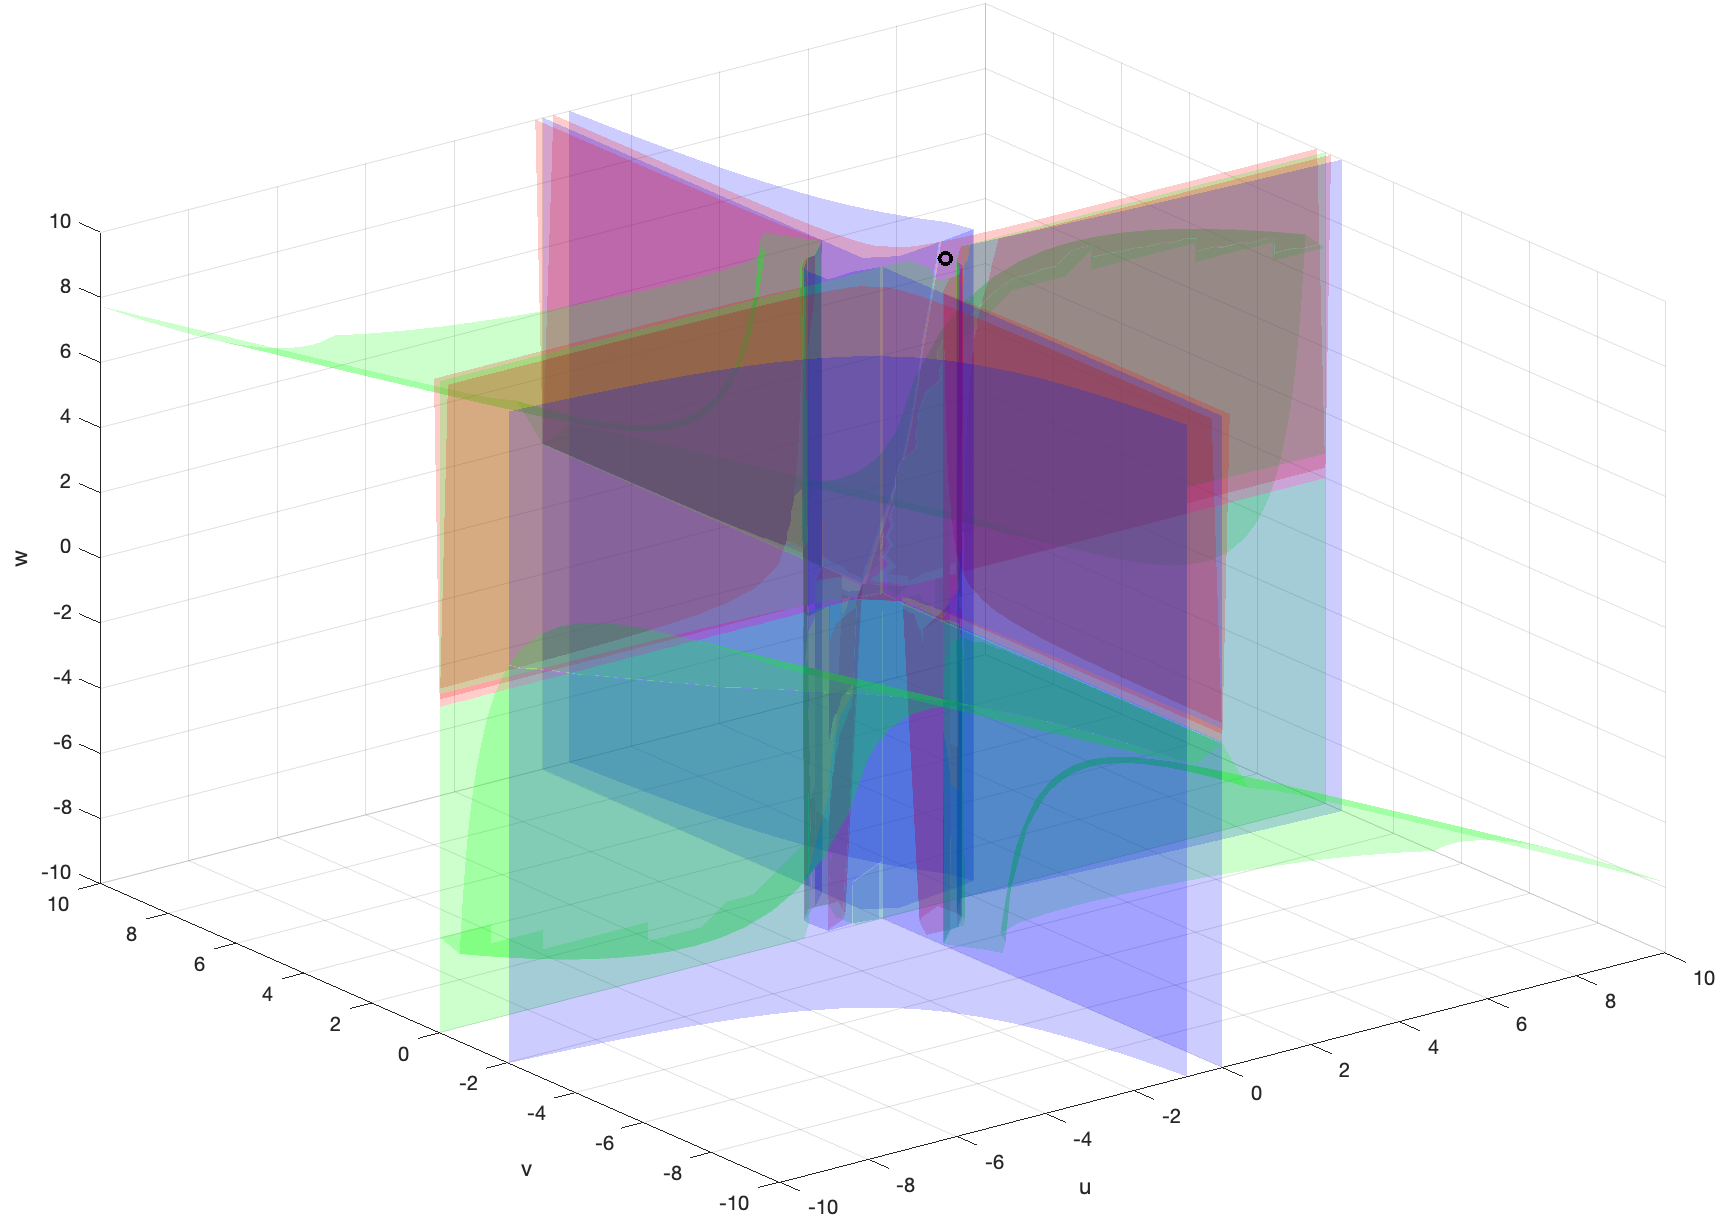
\includegraphics[width=0.49\linewidth]{figures/nullclines.png}
		&
		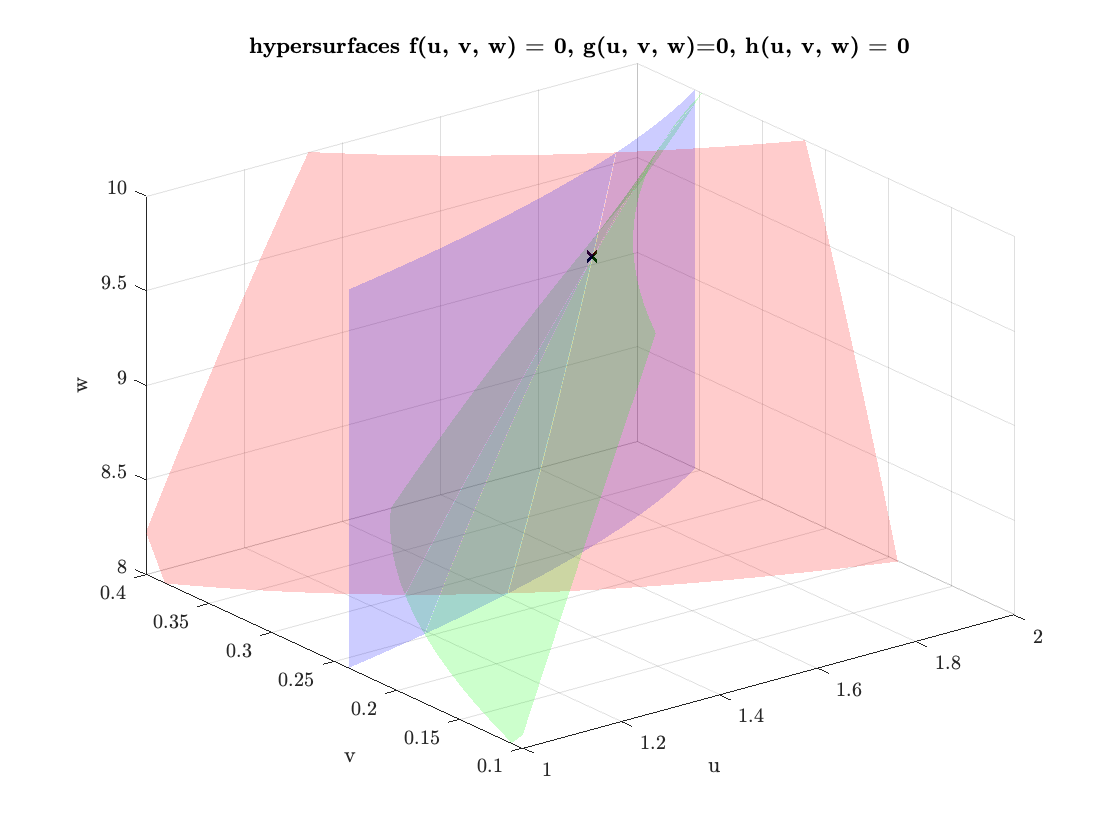
\includegraphics[width=0.49\linewidth]{figures/nullclines_zoom.png}
	\end{tabular}
\caption{Three-dimensional plot of the algebraic hypersurfaces associated to equations $f \equiv 0$ (blue), $g \equiv 0$ (green) and $h \equiv 0$ (red). The choice of parameters $\mu_f = 0.87, \mu_b = 0.68, \mu_l = 0.05, \mu_e = 0.60, m_1 = 5.36, m2 = 9.68, m3 = 17.27$ is made so that three steady-states exist. The figure on the left-hand panel is plotted over the domain $[-10, 10]^3$ while the right-hand panel plotted in a neighborhood of the non-zero stable steady-state.}
\end{figure}

\subsubsection{Analytical expression of constant steady-states}

The strategy here is to first find, if any, functions $\euH$ and $\euG$ such that $\bar u = \euH(\bar v)$ and $\bar w = \euG(\bar v)$ and then derive a condition on $\bar v$ to conclude. We formulate

%\begin{proposition}[Constant stationary solutions]
%	Let $\bar{\bm u} = (\bar u, \bar v, \bar w)$ be a constant steady-state of (\ref{eq:redu})-(\ref{eq:redw}). Then, either $ (\bar u, \bar v, \bar w) = (0, 0, 0)$ or $\bar u = \euH(\bar v), \bar w = \euG(\bar v)$
%	and all possible values of $\bar v$ are given by the roots of $\euP$ where
%	$$\euH(x) = \frac{m_1}{\mu_f + \mu_b x} - \frac{1}{x}, \qquad \euG(x) = \frac{m_3}{\mu_e}\left( 1 - \frac{\mu_f+ \mu_b }{m_1 x} \right), \qquad \euP(x) = ax^3 + bx^2 + cx + d$$
%	and the coefficients of $\euP$ are given by
%	\begin{align*}
%		a &= -\ml \mb - \frac{m_3 \mb}{\me} + \frac{m_3 \mb^2}{m_1 \me}, \\[0.5em]
%		b &= -\ml\mf + m_2\mb - \frac{m_2 \mb^2}{m_1} +\mb^2 - m_1\mb - \frac{m_3 \mf}{\me} + \frac{2 \mf\mb m_3}{\me m_1}, \\[0.5em]
%		c &= m_2\mf - \frac{2\mf\mb m_2}{m_1} + \mf\mb + \frac{m_3 \mf^2}{\me m_1}, \\[0.5em] 
%		d &= -\frac{m_2\mf^2}{m_1}.
%	\end{align*}
%\end{proposition}


\begin{proposition}[Constant stationary solutions]
	Let $\bar{\bm u} = (\bar u, \bar v, \bar w)$ be a constant steady-state of (\ref{eq:redu})-(\ref{eq:redw}). Then, either $ (\bar u, \bar v, \bar w) = (0, 0, 0)$ or $\bar u = \euH(\bar v), \bar w = \euG(\bar v)$
	and all possible values of $\bar v$ are given by the roots of $\euP$ where
	$$\euH(x) = \frac{m_1}{\mu_f + \mu_b x} - \frac{1}{x}, \qquad \euG(x) = \frac{m_3}{\mu_e}\left( 1 - \frac{\mu_f+ \mu_b }{m_1 x} \right)$$
	and  $\euP$ is given by
	
	\begin{multline}
		\euP{(x)} = \biggl(-\ml \mb - \frac{m_3 \mb}{\me} + \frac{m_3 \mb^2}{m_1 \me}\biggr)x^3 \\+ \biggl(-\ml\mf + m_2\mb - \frac{m_2 \mb^2}{m_1} +\mb^2 - m_1\mb - \frac{m_3 \mf}{\me} + \frac{2 \mf\mb m_3}{\me m_1}\biggr)x^2 \\ + \biggl(m_2\mf - \frac{2\mf\mb m_2}{m_1} + \mf\mb + \frac{m_3 \mf^2}{\me m_1}\biggr)x -\frac{m_2\mf^2}{m_1}.
	\end{multline}
\end{proposition}
\begin{proof}
	The proof consists of straightforward computations that are carried out in details in appendix [NOM APPENDIX].
\end{proof}

While this is quite a ludicrous task to achieve, one could derive the exact analytical expression for spatially homogeneous stationary solutions of (\ref{eq:redu})-(\ref{eq:redw}) using the cubic formula and by differentiating cases with positive (negative) discriminant to toss away imaginary roots. An important thing to notice is that some choices of parameters will lead $\euP$ to have roots $v$ such that one coordinate of $\bar{\bm u}$ is negative, or complex-valued. Since we always choose an initial condition $\bm u_0 > 0$, this is contradictory with the results proven in the last section. When this happens, it is an indicator that the system will converge towards the origin instead of another steady-state. \com{maybe try to find parameters such that only one root is positive and two are complex-conjugate, e.g. $(r_1, r_2, r_3) = (3, 1+i, 1-i)$ such that $\euH(r_1), \euG(r_1) > 0$ to see if it is possible to get another steady state that is not the origin.}

\begin{example}[Numerical computations of the roots]
	In MATLAB, we implement the polynomial $\euP$ as well as $\euG$ and $\euH$. We then use the function \texttt{roots} to find all eventual steady states (see figure (\ref{fig:matlabP})).
	\begin{figure}
		\label{fig:matlabP}
		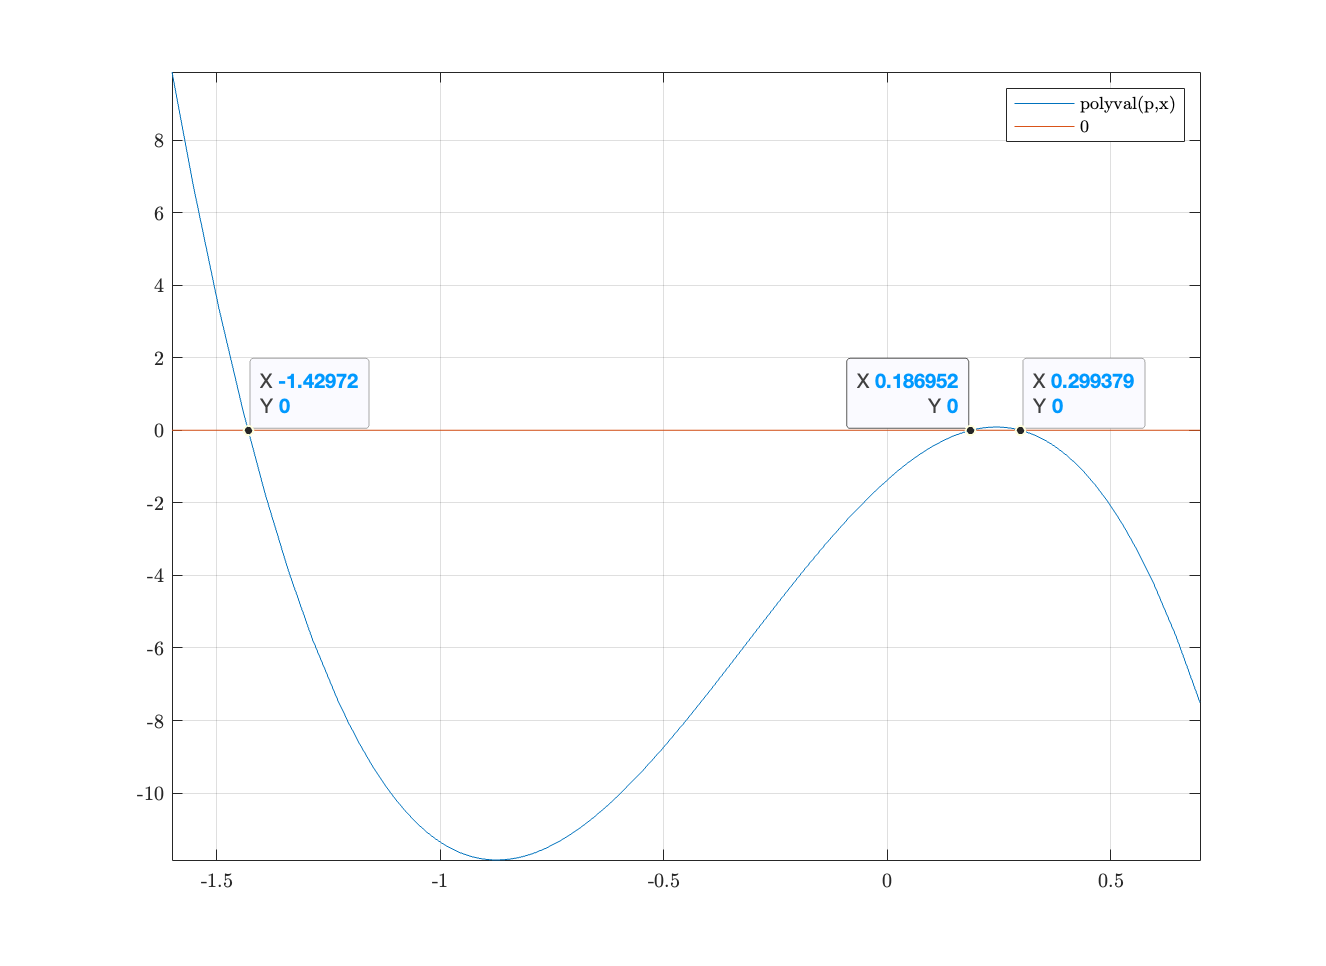
\includegraphics[width=0.6\linewidth]{figures/polyP_v.png}
		\caption{Roots of $\euP$ for $\mu_f = 0.87$, $\mu_b = 0.68$, $\mu_l = 0.05$, $\mu_e = 0.60$, $m_1 = 5.36$, $m2 = 9.68$, $m3 = 17.27$ (same parameters as in figure (\ref{fig:nullclines})) }
	\end{figure}
	Using the exact values returned by the machine, we find four steady-states 
	$$\bar{\bm u}_{3} = (0, 0, 0), \quad \bar{\bm u}_{2} = (-51.6587, -1.4300, 28.3989) $$
	$$\bar{\bm u}_{3} = (1.6527, 0.2994, 9.5284), \quad \bar{\bm u}_{4} = (0.0138, 0.1864, 0.0739)$$
	As previously mentioned, we can rule out $\bar{\bm u}_2$ because it has at least one negative coordinate. From there, using the Jacobian (computed in the next section) we can deduce the nature of $\bar{\bm u}_1, \bar{\bm u}_3, \bar{\bm u}_4$ and it reveals that the origin and $\bar{\bm u}_3$ are stable while $\bar{\bm u}_4$ is unstable.
\end{example}
	
	

\subsubsection{Snack break: finding bounds on asymptotically stable spatially homogeneous stationary solutions}

hey hey


\subsection{Linear dynamics and local behavior of the system}

In order to meet the required conditions for DDI, we first have to make sure system (\ref{eq:redu})-(\ref{eq:redw}) is stable in absence of diffusion when computed at a spatially homogeneous steady-state. This translates into saying that the Jacobian matrix $J = J_{\bm f}(u, v, w)$ of $\bm f$ at a steady-state satisfies $s(J) < 0$. A rapid computation shows

$$
J = \bpm  -\mu_f +  \dfrac{m_1v}{(1+u v)^2} - \mu_b v &  \dfrac{m_1 u}{(1+u v)^2} - \mu_b u & 0 \\[1.2em]
 \dfrac{m_2 v}{(1+u v)^2} - \mu_b v   & -\mu_l + \dfrac{m_2 u}{(1+u v)^2} - \mu_b u - w  & -v \\[1.2em] 
  \dfrac{m_3 v}{(1+u v)^2} &  \dfrac{m_3 v}{(1+u v)^2} & -\mu_e \epm.
$$

When working around the origin, it is perfectly fine to work with $J$ as it is. However, this form turns out to be rather impractical to work with when carrying out later computations around the other non-zero steady state. As a parry, we will later derive a set of useful equalities that will help us simplify the expression of $J$.

\subsubsection{In a neighborhood of the origin}

When taking $(u, v, w) = (0, 0, 0)$, almost all terms in the Jacobian disappear, leaving us with

$$
A(0, 0, 0) = \bpm  -\mu_f  &  0 & 0 \\[1.2em]
0  & -\mu_l & 0 \\[1.2em] 
0 & 0 & -\mu_e \epm
$$

which, by positivity of $\mu_f, \mu_b, \mu_e$ is unconditionally stable. Take a moment to convince yourself that in this case, there is no hope for DDI (to see why, notice that $\tr (A-\bm\mu D) < 0$ and $\det (A-\bm\mu D) = -\mu_f(\mu_l+ \bm\mu / \gamma)(\mu_e + \bm\mu d_2 / \gamma) < 0$ for all non-negative choices of $\bm\mu$). This tells us the system will always be stable, a statement that is corroborated by running a few simulations (see figure \ref{fig:simulations}).

\begin{figure}
	\centering
	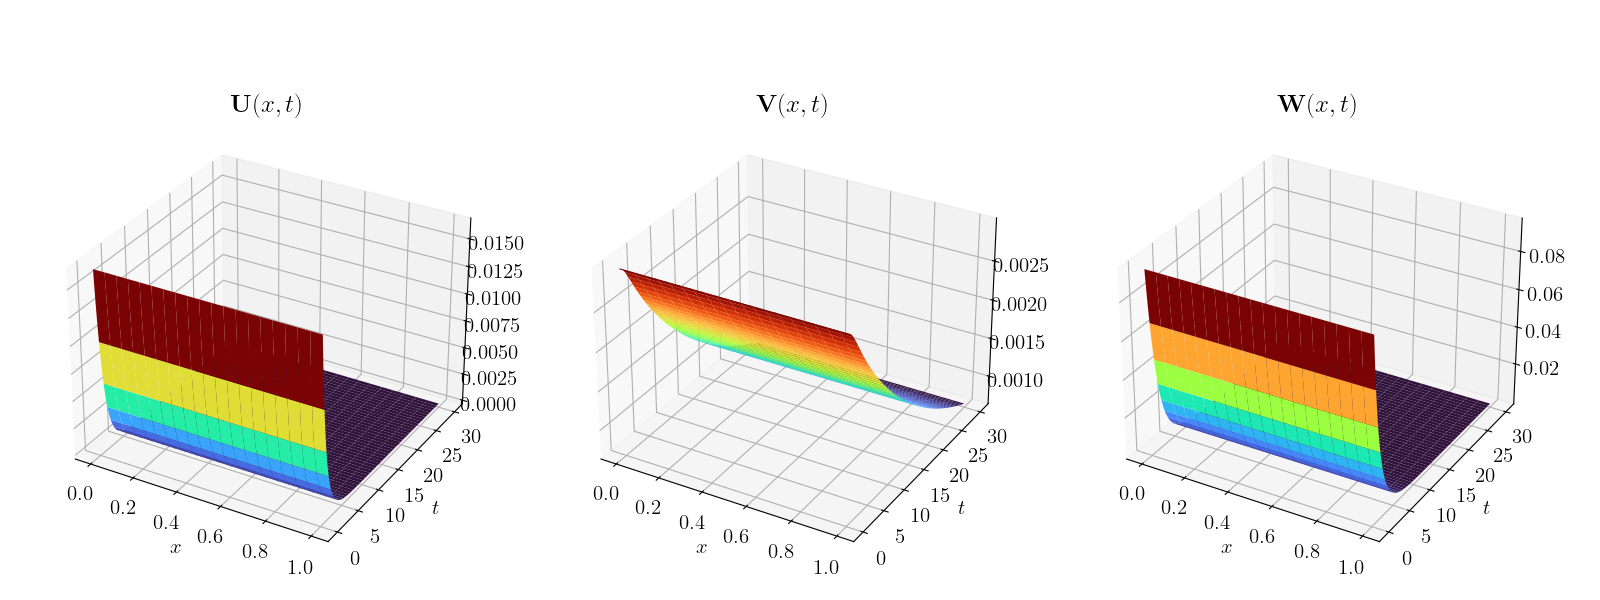
\includegraphics[width=\textwidth]{figures/stable_origin.png}
	\caption{space-time plot of numerical solutions $u, v, w$ to \ref{eq:system} with constant initial condition $\bm X_0 = (\uu_0, \vv_0, \ww_0)$ close to the origin. One clearly sees how each quantity converges towards 0}
	\label{fig:simulations}
\end{figure}

\subsubsection{Around the other steady state}

Let us move our interest to the other stable steady state (provided the choice of parameters allows it to exist). Using the fact that each term $u, v, w$ is positive, we can operate some surgery on identities \ref{identities} to derive

\begin{equation}
	\label{new_identities}
		m_1 \dfrac{v}{1 + u v} = \mu_f +  \mu_b v \quad \quad
		m_2 \dfrac{u}{1 + u v}  = \mu_l +  \mu_b u + w \quad \quad
		m_3 \dfrac{ u v}{1 + uv} = \mu_e w
\end{equation}


\begin{theorem}[Routh-Hurwitz criterion of order 3]
	Take a matrix $M \in \euM_3(\R)$. Then all the roots of $\chi_M$ lie in the negative half-plane (i.e. $\sigma(M) \subset \R_{<0}$) if and only if
	$\Delta_i(M) > 0$ for $i=1, 2, 3$ holds, where we define
	\begin{align*}
		\Delta_1(M) &= -\tr(M) \\[0.7em]
		\Delta_2(M) &= -\tr(M) \sum_{i < j} \det(M_{ij}) + \det(M) \\[0.7em]
		\Delta_3(M) &= -\det(M) \Delta_2(M),
	\end{align*}
Alternatively, let $\Tilde{\chi}_{M}(\lambda) = a_0 + a_1 \lambda + a_2 \lambda^2 + \lambda^3$ be the normalized characteristic polynomial of $M$. Then all roots of $\Tilde{\chi}_M$ lie in the negative half-plane if and only if all coefficients are positive and $a_2 a_1 > a_0$.
\end{theorem}


\begin{definition}[Submatrices defined by a pair of indices]
	Consider a matrix $A \in \euM_n(\R)$, for any couple of distinct indices $(i, j)$ with $1 \le i, j \le n$, we introduce the notation $A_{ij}$ to be the $2 \! \times \! 2$-matrix whose entries are formed by the entries of $A$ on line and column $i, j$.
\end{definition}


\begin{proposition}[Characteristic polynomial of a $3\times3$ matrix] Consider a matrix $A \in \euM_3(\R)$ whose entries are the $a_{ij}$ for $1 \le i, j \le 3$. Then 
	$$\chi_A(\lambda) = -\lambda^3 + \tr(A) \lambda^2 - \lp \sum_{i < j} \det(A_{ij})\rp \lambda + \det(A)$$.
\end{proposition}


\begin{lemma}[Necessary condition for DDI] Let $B := A - \lambda D$ denote the matrix of the linearized system. We claim that we obtain DDI if and only if $\det(B_{12}) < 0$ and 
	
\end{lemma}


\begin{remark}[Minimum] The function $\mu \longmapsto |A - \mu D|$ reaches its minimum at the point:
	
\begin{equation}
	\resizebox{\hsize}{!}{%
		$\mu_{\mathbf{\mathrm{min}}} = \dfrac{\gamma}{2}\left( \dfrac{1}{(1+uv)^2}\left( m_2 u -  \dfrac{m_1m_2uv + \mu_b^2 uv(1+uv)^4 - \mu_b(m_1 + m_2) uv(1+uv)^2}{m_1 v - \mu_f (1 + uv)^2 - \mu_b v(1+uv)^2} \right)-\dfrac{\mu_e}{d_2} - \mu_l - \mu_b u - w\right) \notag$  
	}
\end{equation}
Please do not make me compute $\det(A - \mu_{\textrm{min}} D)$ ;-;. Also
\begin{equation}
	\resizebox{\hsize}{!}{%
		$\mu_{\mathbf{\mathrm{min}}} > 0 \quad \iff\quad \mu_f \biggl(m_2 - \mu_b u (1 + uv)^2\biggr) > \left( \dfrac{\mu_e}{d_2} + \mu_l + w \right) \biggl( m_1 v - \mu_f(1+uv)^2 - \mu_b v (1 + uv)^2\biggr) \notag$  
	}
\end{equation}
\end{remark}



$$\frac{|A_{12}| + |A_{13}|d_2}{2a_{11} d_2}$$



%
\section{From Operator Semigroups to Spectral Theory}
\label{app:SpecTheo}

(\com{Maybe put this section in Appendix})
In this section, we introduce classical results from semigroup and spectral theory to prove that the RD system has solutions under relatively weak assumptions.


The system can be rewritten more generally under the form

$$\left\{\begin{aligned}
& \del_t \xi = L \xi + N(\xi)  \quad &\xi = (\bm u, \bm v) - (\bar{\bm u}, \bar{\bm v})  \\[1em]
& \xi(0, x) \in L^\infty(\Omega)^m \times L ^{\infty}(\Omega)^k    
\end{aligned}
\right.
$$

With the linear operator part of the system

$$L \xi = \bpm \bm{0} & \bm{0} \\ \bm{0}& D\epm \lap \xi + \bpm j_{11} & j_{12} \\ j_{21} & j_{22} \epm \xi $$
and the non-linear part being the terms of order $\ge2$ in the expansion of $\xi$


\begin{definition}[spectral bound]
    Let $L$ be an operator with spectrum $\sigma(L)$, then, the spectral bound $s(L)$ is defined by
    $$s(L) = \sup \lc \re(\lambda) : \lambda \in \sigma(L) \rc$$
\end{definition}
\bigskip

\begin{definition}[Growth Exponent]
    We call the growth exponent of an exponentially bounded $\mathcal{C}^0$-semigroup $(T(t))_{t\ge 0}$ the real number $w$ defined by

    $$w = \inf_{\R} \bl\{ w : \exists M > 1, \forall t \ge 0, ||T(t)|| \le Me^{wt} \br\}$$
\end{definition}
\bigskip

\begin{proposition}[Generated Semigroups]
The operator $L$ generates an analytic $\mathcal C^0$-semigroup $(T(t))_{t\ge 0}$ through the map $t \longmapsto \exp(tL)$. The system $\del_t \xi = L\xi$ is therefore linearly stable if the growth exponent $w < 0$. It is linearly unstable otherwise.
\end{proposition}

\begin{definition}[Mild solutions]
    Let $X$ be a Banach space and take $L$, the infinitesimal generator of a $\mathcal C^0$-semigroup $(T(t))_{t\ge 0}$. Let $\xi : I \times \Omega \longrightarrow \R^{m+k}$ such that $\xi(t, \cdot) \in X$. The function $\xi$ is said to be a mild solution of the system if it obeys
    $$\xi(t, \cdot) = T(t)\xi(0, \cdot) + \int_{0}^{t} T(t- \tau) \xi(\tau, \cdot) d\tau$$
\end{definition}


\section{Conditions Required for Diffusion Driven Instabilities (DDI)}
\label{app:Turing}

We provide a set of conditions for one to obtain DDI for a $n$-dimensional reaction diffusion  (RD). Such systems are often represented under the form
$$\del_t u - D \lap u = F(U)$$
with $u \in \R^n$, $D \in \euM_n(\R)$ and $F \in \mathcal C^1(\R^n, \R^n)$. Let $\bar u$ be a constant equilibrium of the system and introduce $B := \mathcal J_F(\bar u)$ the Jacobian matrix of $F$ computed at the steady-state $\bar u$. Consider a small perturbation $\xi := u - \bar u \in \R^n$ around the steady state and linearize the system around $\bar u$.
$$\del_t \xi - D \lap \xi = B \xi $$
Now look for solutions of the form $\xi(x, t) = e^{\lambda t} \Phi(x)$ yields $D\lap \Phi + (B - \lambda) \Phi = 0$. We then decompose $\Phi = \sum_{m \ge 0} y_m \varphi_m(x)$ in the basis composed of eigenfunctions of the Laplacian with Neumann boundary conditions.


%
\section{Deriving the model for Hydra (finding kinetics and explaining MM term)}

\subsection{Derivation of the model}

\subsection{Model reduction}

\subsubsection{Quasi steady-state approximation}

\com{make the start of this section match with the end of the previous one} The purpose of this section is to take the equations we have derived and reduce the dimensionality by approximating the quantity $r_b$ \textit{via} quasi steady-state (QSS) approximation. 
% So far, the model can be written as follows
% 
% \be
% \label{eq:Model4Vars}
% \bc
%     \del_t \bm{u} &= -\mu_f \bm{u} + m_1 \dfrac{\bm{r_b}}{1 + \bm{r_b}} - b \bm{u} \bm{v} + d \bm{r_b} \\[0.9em]
%     \del_t \bm{r_b} &= -\mu_b \bm{r_b} + b \bm{u} \bm{v} - d \bm{r_b} \\[0.9em]
%     \del_t \bm{v} &= \dfrac{1}{\gamma} \delxx{\bm{v}} - \mu_l \bm{v} + m2 \dfrac{\bm{r_b}}{1 + \bm{r_b}} - b \bm{u} \bm{v} + d \bm{r_b} - b_e \bm{v} \bm{r_e} \\[0.9em]
%     \del_t \bm{w} &= \dfrac{d_2}{\gamma} \delxx{\bm{w}} - \mu_e \bm{w} + m_3 \dfrac{\bm{r_b}}{1 + \bm{r_b}}
% \ec
% \ee
% \bigskip

The quasi steady-state approximation yields
$\bm{r_b} = \alpha \bm{u} \bm{v}$ and $\alpha = b / (d + \mu_b)$. With that, $\bm{r_b}$ is now out of the differential system and algebraic surgery on each equation leads to 
\be
\bc
    \del_t \uu &= -\mu_f \uu + m_1 \dfrac{\alpha \uu \vv}{1 + \alpha \uu \vv} - b \uu \vv + d \alpha \uu \vv \\[0.9em]
    \del_t \vv &= \dfrac{1}{\gamma} \delxx{\vv} - \mu_l \vv + m_2 \dfrac{\alpha \uu \vv}{1 + \alpha \uu\vv} - b \uu \vv + d \alpha \uu \vv - b_e \vv\ww \\[0.9em]
    \del_t \ww &= \dfrac{d_2}{\gamma} \delxx{\ww} - \mu_e \ww + m_3 \dfrac{\alpha\uu\vv}{1 + \alpha\uu\vv}
\ec
\ee
\bigskip
Additionally, we suggest the following rescaling for the quantities involved in the model. 
\begin{center}
\begin{tabular}{|c|c|c|c|c|c|c|c|}
\hline
Old variable & $\Tilde{\ww}$ & $\Tilde{\uu}$ &  $\Tilde{\vv}$ & $\Tilde{m_1}$ & $\Tilde{m_2}$ & $\Tilde{m_3}$ & $\Tilde{\mu_b}$
\\ \hline
New variable & $b_e \ww$ & 
$\sqrt{\alpha} \uu$ &
$\sqrt{\alpha} \vv$ & 
$\sqrt{\alpha} m_1$ &
$\sqrt{\alpha} m_2$ &
$b_e m_3$ &
$\sqrt{\alpha} \mu_b$ \\ \hline
\end{tabular}    
\end{center}
Which altogether leads to
\be
\bc
    \del_t \uu &= -\mu_f \uu + \Tilde{m_1} \dfrac{\uu \vv}{1 +\uu \vv} - \Tilde{\mu_b} \uu \vv \\[0.9em]
    \del_t \vv &= \dfrac{1}{\gamma} \delxx{\vv} - \mu_l \vv + \Tilde{m_2} \dfrac{\uu \vv}{1 + \uu\vv} - \Tilde{\mu_b} \uu \vv -\vv\ww \\[0.9em]
    \del_t \ww &= \dfrac{d_2}{\gamma} \delxx{\ww} - \mu_e \ww + \Tilde{m_3} \dfrac{\uu\vv}{1 + \uu\vv}
\ec
\ee
\bigskip


\newpage

\appendix






\nocite{*}
\printbibliography

\end{document}